\documentclass[12pt,a4paper]{article}
\usepackage[utf8]{vietnam}
\usepackage{amsmath,amssymb}
\usepackage{tabularx}
\usepackage{tikz}
\usepackage{xcolor}
\usepackage[top=0.6cm, bottom=0.6cm, left=0.6cm, right=0.6cm]{geometry}
\usepackage[dethi]{ex_test}

\SAOPTN{widthSA=2.6,heightSA=0.62}
\setlength{\parskip}{0pt}

% Dong ke cham mo chuan viet tay
\newcommand{\dongke}[1]{%
  \begingroup%
  \setlength{\parskip}{0pt}%
  \baselineskip=18.5pt%
  \vspace{1.0mm}%
  \foreach \i in {1,...,#1}{%
    \noindent{\color{gray!60}\dotfill}\par%
  }%
  \vspace{0.6mm}%
  \endgroup%
}

% Khu vuc bai lam chia 2 cot co vach ngan mo o giua
\newcommand{\dongkeHaiCot}[1]{%
  \par\vspace{0.5mm}%
  \noindent%
  \begin{minipage}[t]{0.485\linewidth}%
    \dongke{#1}%
  \end{minipage}%
  \hfill%
  {\color{gray!60}\vrule}%
  \hfill%
  \begin{minipage}[t]{0.485\linewidth}%
    \dongke{#1}%
  \end{minipage}%
}

% Dinh nghia o bai tap tu luan trong bang
\newcommand{\oBaiTap}[3][5]{%
  \vspace{1.0mm}%
  \noindent\textbf{#2} #3\par%
  \dongke{#1}%
}

\begin{document}
\pagestyle{empty}
% =============================================================================
% ========================= TOAN 7 TUAN 09 BUOI 02 - MA DE 101 =================
% ========================= TRANG 1/2 ==========================================
% =============================================================================
\noindent
\begin{tabularx}{\linewidth}{|X|c|}
\hline
\textbf{PHIẾU KIỂM TRA ĐỊNH KỲ TOÁN 7 - TUẦN 09 - BUỔI 02} & \textbf{Mã đề: 101 - Trang 1/2} \\
\hline
\end{tabularx}

\vspace{1.2mm}

\noindent
\begin{tabularx}{\linewidth}{|p{3.2cm}|X|}
\hline
\centering\textbf{ĐIỂM SỐ} & \centering\textbf{LỜI NHẬN XÉT CỦA THẦY CÔ} \tabularnewline
\hline
\rule{0pt}{1.8cm} & \tabularnewline
\hline
\end{tabularx}

\vspace{1.5mm}
\noindent\textbf{Câu 1 (0,25 điểm).} Số đối của số hữu tỉ $\dfrac{4}{7}$ là: \shortans{-\dfrac{4}{7}}\par\vspace{2.7mm}
\noindent\textbf{Câu 2 (0,25 điểm).} Giá trị của căn bậc hai số học $\sqrt{81}$ bằng: \shortans{9}\par\vspace{2.7mm}
\noindent\textbf{Câu 3 (0,25 điểm).} Giá trị của biểu thức $|-6{,}2|$ bằng: \shortans{6{,}2}\par\vspace{2.7mm}
\noindent\textbf{Câu 4 (0,25 điểm).} Mỗi góc ngoài của một tam giác có số đo bằng: \shortans{\text{tổng 2 góc trong không kề}}\par\vspace{2.7mm}
\noindent\textbf{Câu 5 (0,25 điểm).} Cho $\Delta ABC$ có $\widehat{A} = 45^\circ, \widehat{B} = 65^\circ$. Số đo góc ngoài tại đỉnh $C$ là: \shortans{110^\circ}\par\vspace{2.7mm}
\noindent\textbf{Câu 6 (0,25 điểm).} Góc ngoài tại đỉnh $A$ của $\Delta ABC$ bằng $125^\circ$, biết $\widehat{B} = 55^\circ$. Số đo $\widehat{C}$ là: \shortans{70^\circ}\par\vspace{2.7mm}
\noindent\textbf{Câu 7 (0,25 điểm).} Tổng số đo ba góc ngoài tại ba đỉnh của tam giác bất kì là: \shortans{360^\circ}\par\vspace{2.7mm}
\noindent\textbf{Câu 8 (0,25 điểm).} Cho $\Delta MNP$ vuông tại $M$, góc ngoài tại đỉnh $N$ bằng $140^\circ$. Số đo góc $\widehat{P}$ là: \shortans{50^\circ}\par\vspace{2.7mm}
\noindent\textbf{Câu 9 (0,25 điểm).} Cho $\Delta ABC$ có $\widehat{A} = 70^\circ$, hai phân giác trong góc $B, C$ cắt nhau tại $I$. Số đo $\widehat{BIC}$ là: \shortans{125^\circ}\par\vspace{2.7mm}
\noindent\textbf{Câu 10 (0,25 điểm).} Mái nhà tam giác cân góc đỉnh $100^\circ$. Góc ngoài tại đỉnh ở chân mái bằng: \shortans{140^\circ}\par\vspace{2.7mm}
\vspace{0.2mm}
\noindent\textbf{Câu 11 (3,0 điểm). Thực hiện phép tính (hợp lý nếu có thể):}
\vspace{0.8mm}

\noindent
\begin{tabularx}{\linewidth}{|X|X|}
\hline
\oBaiTap[5]{a) (0,5 điểm)}{$\dfrac{5}{8} + \dfrac{3}{4} - \dfrac{1}{2}$} & 
\oBaiTap[5]{b) (0,5 điểm)}{$\dfrac{5}{12} \cdot \left(-\dfrac{3}{8}\right) + \dfrac{5}{12} \cdot \left(-\dfrac{5}{8}\right)$} \\
\hline
\oBaiTap[5]{c) (0,5 điểm)}{$\left(-\dfrac{2}{3}\right)^2 \cdot \dfrac{9}{8} - \sqrt{\dfrac{1}{4}}$} & 
\oBaiTap[5]{d) (0,5 điểm)}{$\left|-\dfrac{5}{6}\right| - \sqrt{\dfrac{4}{9}} + \dfrac{1}{3}$} \\
\hline
\oBaiTap[5]{e) (0,5 điểm)}{$\dfrac{7}{3} - \left[\dfrac{5}{6} - \left(\dfrac{2}{3} - \dfrac{1}{2}\right)\right]$} & 
\oBaiTap[5]{f) (0,5 điểm)}{$\dfrac{3^8 \cdot 5^4}{15^3 \cdot 9^2}$} \\
\hline
\end{tabularx}

\newpage
% =============================================================================
% ========================= TOAN 7 TUAN 09 BUOI 02 - MA DE 101 =================
% ========================= TRANG 2/2 ==========================================
% =============================================================================
\noindent
\begin{tabularx}{\linewidth}{|X|c|}
\hline
\textbf{TOÁN 7 - TUẦN 09 - BUỔI 02} & \textbf{Mã đề: 101 - Trang 2/2} \\
\hline
\end{tabularx}

\vspace{1.5mm}

\noindent\textbf{Câu 12 (2,0 điểm). Tìm số hữu tỉ $x$, biết:}
\vspace{0.8mm}

\noindent
\begin{tabularx}{\linewidth}{|X|X|}
\hline
\oBaiTap[5]{a) (0,5 điểm)}{$x + \dfrac{4}{7} = \dfrac{11}{14}$} & 
\oBaiTap[5]{b) (0,5 điểm)}{$\dfrac{3}{4}x - \dfrac{1}{3} = \dfrac{5}{12}$} \\
\hline
\oBaiTap[5]{c) (0,5 điểm)}{$\left(x + \dfrac{1}{2}\right)^2 = \dfrac{9}{16}$} & 
\oBaiTap[5]{d) (0,5 điểm)}{$\left|3x - \dfrac{1}{4}
ight| = \dfrac{5}{4}$} \\
\hline
\end{tabularx}

\vspace{1.5mm}

\noindent
\begin{tabularx}{\linewidth}{|X|}
\hline
\vspace{0.5mm}
\begin{minipage}[t]{0.67\linewidth}
\vspace{0pt}
\textbf{Câu 13 (2,0 điểm).} Cho tam giác $ABC$ có $\widehat{A} = 80^\circ$. Hai tia phân giác của hai góc trong $\widehat{B}$ và $\widehat{C}$ cắt nhau tại điểm $I$.\par\vspace{0.4mm}
\textbf{a)} (1,0 điểm) Tính số đo góc $\widehat{BIC}$.\par\vspace{0.4mm}
\textbf{b)} (1,0 điểm) Kéo dài cạnh $AB$ về phía $B$ được tia $Bx'$, kéo dài $AC$ về phía $C$ được tia $Cy'$. Hai tia phân giác của hai góc ngoài $\widehat{x'BC}$ và $\widehat{y'CB}$ cắt nhau tại điểm $K$. Tính số đo góc $\widehat{BKC}$.
\end{minipage}\hfill
\begin{minipage}[t]{0.31\linewidth}
\vspace{0pt}\centering
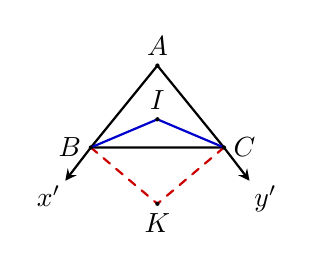
\begin{tikzpicture}[scale=0.65, >=stealth, line join=round, line cap=round]
  \coordinate (A) at (1.5, 2.3);
  \coordinate (B) at (0.2, 0.7);
  \coordinate (C) at (2.8, 0.7);
  \coordinate (I) at (1.5, 1.25);
  \coordinate (K) at (1.5, -0.4);
  
  \draw[thick] (A) -- (B) -- (C) -- cycle;
  \draw[thick, blue!80!black] (B) -- (I) -- (C);
  
  \draw[thick, ->] (B) -- (-0.3, 0.05) node[below left=-2pt] {$x'$};
  \draw[thick, ->] (C) -- (3.3, 0.05) node[below right=-2pt] {$y'$};
  
  \draw[thick, red!80!black, dashed] (B) -- (K) -- (C);
  
  \fill (A) circle (1.2pt) node[above] {$A$};
  \fill (B) circle (1.2pt) node[left] {$B$};
  \fill (C) circle (1.2pt) node[right] {$C$};
  \fill (I) circle (1.2pt) node[above] {$I$};
  \fill (K) circle (1.2pt) node[below] {$K$};
\end{tikzpicture}
\end{minipage}\par
\vspace{0.4mm}
\noindent\textit{Bài giải:}\dongkeHaiCot{9}
\\ \hline
\end{tabularx}

\vspace{1.5mm}

\noindent
\begin{tabularx}{\linewidth}{|X|}
\hline
\vspace{0.5mm}
\textbf{Câu 14 (0,5 điểm).} Tìm giá trị lớn nhất của biểu thức: $B = \dfrac{12}{|x - 3| + 4}$.\par
\vspace{0.4mm}
\noindent\textit{Bài giải:}\dongkeHaiCot{7}
\\ \hline
\end{tabularx}

\newpage
% =============================================================================
% ========================= TOAN 7 TUAN 09 BUOI 02 - MA DE 102 =================
% ========================= TRANG 1/2 ==========================================
% =============================================================================
\noindent
\begin{tabularx}{\linewidth}{|X|c|}
\hline
\textbf{PHIẾU KIỂM TRA ĐỊNH KỲ TOÁN 7 - TUẦN 09 - BUỔI 02} & \textbf{Mã đề: 102 - Trang 1/2} \\
\hline
\end{tabularx}

\vspace{1.2mm}

\noindent
\begin{tabularx}{\linewidth}{|p{3.2cm}|X|}
\hline
\centering\textbf{ĐIỂM SỐ} & \centering\textbf{LỜI NHẬN XÉT CỦA THẦY CÔ} \tabularnewline
\hline
\rule{0pt}{1.8cm} & \tabularnewline
\hline
\end{tabularx}

\vspace{1.5mm}
\noindent\textbf{Câu 1 (0,25 điểm).} Số đối của số hữu tỉ $\dfrac{3}{8}$ là: \shortans{-\dfrac{3}{8}}\par\vspace{2.7mm}
\noindent\textbf{Câu 2 (0,25 điểm).} Giá trị của căn bậc hai số học $\sqrt{144}$ bằng: \shortans{12}\par\vspace{2.7mm}
\noindent\textbf{Câu 3 (0,25 điểm).} Giá trị của biểu thức $|-4{,}8|$ bằng: \shortans{4{,}8}\par\vspace{2.7mm}
\noindent\textbf{Câu 4 (0,25 điểm).} Mỗi góc ngoài của một tam giác có số đo bằng: \shortans{\text{tổng 2 góc trong không kề}}\par\vspace{2.7mm}
\noindent\textbf{Câu 5 (0,25 điểm).} Cho $\Delta ABC$ có $\widehat{A} = 55^\circ, \widehat{B} = 50^\circ$. Số đo góc ngoài tại đỉnh $C$ là: \shortans{105^\circ}\par\vspace{2.7mm}
\noindent\textbf{Câu 6 (0,25 điểm).} Góc ngoài tại đỉnh $A$ của $\Delta ABC$ bằng $130^\circ$, biết $\widehat{B} = 65^\circ$. Số đo $\widehat{C}$ là: \shortans{65^\circ}\par\vspace{2.7mm}
\noindent\textbf{Câu 7 (0,25 điểm).} Tổng số đo ba góc ngoài tại ba đỉnh của tam giác bất kì là: \shortans{360^\circ}\par\vspace{2.7mm}
\noindent\textbf{Câu 8 (0,25 điểm).} Cho $\Delta MNP$ vuông tại $M$, góc ngoài tại đỉnh $N$ bằng $135^\circ$. Số đo góc $\widehat{P}$ là: \shortans{45^\circ}\par\vspace{2.7mm}
\noindent\textbf{Câu 9 (0,25 điểm).} Cho $\Delta ABC$ có $\widehat{A} = 60^\circ$, hai phân giác trong góc $B, C$ cắt nhau tại $I$. Số đo $\widehat{BIC}$ là: \shortans{120^\circ}\par\vspace{2.7mm}
\noindent\textbf{Câu 10 (0,25 điểm).} Mái nhà tam giác cân góc đỉnh $110^\circ$. Góc ngoài tại đỉnh ở chân mái bằng: \shortans{145^\circ}\par\vspace{2.7mm}
\vspace{0.2mm}
\noindent\textbf{Câu 11 (3,0 điểm). Thực hiện phép tính (hợp lý nếu có thể):}
\vspace{0.8mm}

\noindent
\begin{tabularx}{\linewidth}{|X|X|}
\hline
\oBaiTap[5]{a) (0,5 điểm)}{$\dfrac{3}{10} + \dfrac{4}{5} - \dfrac{1}{2}$} & 
\oBaiTap[5]{b) (0,5 điểm)}{$\dfrac{7}{15} \cdot \left(-\dfrac{4}{9}\right) + \dfrac{7}{15} \cdot \left(-\dfrac{5}{9}\right)$} \\
\hline
\oBaiTap[5]{c) (0,5 điểm)}{$\left(-\dfrac{3}{4}\right)^2 \cdot \dfrac{16}{9} - \sqrt{\dfrac{9}{16}}$} & 
\oBaiTap[5]{d) (0,5 điểm)}{$\left|-\dfrac{7}{8}\right| - \sqrt{\dfrac{25}{64}} + \dfrac{1}{4}$} \\
\hline
\oBaiTap[5]{e) (0,5 điểm)}{$\dfrac{8}{3} - \left[\dfrac{7}{6} - \left(\dfrac{3}{4} - \dfrac{1}{4}\right)\right]$} & 
\oBaiTap[5]{f) (0,5 điểm)}{$\dfrac{2^8 \cdot 7^4}{14^3 \cdot 4^2}$} \\
\hline
\end{tabularx}

\newpage
% =============================================================================
% ========================= TOAN 7 TUAN 09 BUOI 02 - MA DE 102 =================
% ========================= TRANG 2/2 ==========================================
% =============================================================================
\noindent
\begin{tabularx}{\linewidth}{|X|c|}
\hline
\textbf{TOÁN 7 - TUẦN 09 - BUỔI 02} & \textbf{Mã đề: 102 - Trang 2/2} \\
\hline
\end{tabularx}

\vspace{1.5mm}

\noindent\textbf{Câu 12 (2,0 điểm). Tìm số hữu tỉ $x$, biết:}
\vspace{0.8mm}

\noindent
\begin{tabularx}{\linewidth}{|X|X|}
\hline
\oBaiTap[5]{a) (0,5 điểm)}{$x + \dfrac{3}{5} = \dfrac{9}{10}$} & 
\oBaiTap[5]{b) (0,5 điểm)}{$\dfrac{2}{5}x - \dfrac{1}{2} = \dfrac{1}{10}$} \\
\hline
\oBaiTap[5]{c) (0,5 điểm)}{$\left(x + \dfrac{1}{3}\right)^2 = \dfrac{4}{9}$} & 
\oBaiTap[5]{d) (0,5 điểm)}{$\left|2x - \dfrac{1}{4}
ight| = \dfrac{7}{4}$} \\
\hline
\end{tabularx}

\vspace{1.5mm}

\noindent
\begin{tabularx}{\linewidth}{|X|}
\hline
\vspace{0.5mm}
\begin{minipage}[t]{0.67\linewidth}
\vspace{0pt}
\textbf{Câu 13 (2,0 điểm).} Cho tam giác $ABC$ có $\widehat{A} = 70^\circ$. Hai tia phân giác của hai góc trong $\widehat{B}$ và $\widehat{C}$ cắt nhau tại điểm $I$.\par\vspace{0.4mm}
\textbf{a)} (1,0 điểm) Tính số đo góc $\widehat{BIC}$.\par\vspace{0.4mm}
\textbf{b)} (1,0 điểm) Kéo dài cạnh $AB$ về phía $B$ được tia $Bx'$, kéo dài $AC$ về phía $C$ được tia $Cy'$. Hai tia phân giác của hai góc ngoài $\widehat{x'BC}$ và $\widehat{y'CB}$ cắt nhau tại điểm $K$. Tính số đo góc $\widehat{BKC}$.
\end{minipage}\hfill
\begin{minipage}[t]{0.31\linewidth}
\vspace{0pt}\centering
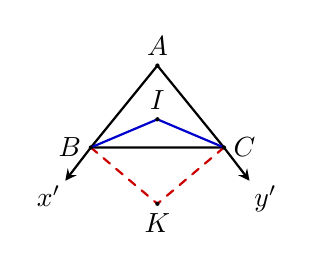
\begin{tikzpicture}[scale=0.65, >=stealth, line join=round, line cap=round]
  \coordinate (A) at (1.5, 2.3);
  \coordinate (B) at (0.2, 0.7);
  \coordinate (C) at (2.8, 0.7);
  \coordinate (I) at (1.5, 1.25);
  \coordinate (K) at (1.5, -0.4);
  
  \draw[thick] (A) -- (B) -- (C) -- cycle;
  \draw[thick, blue!80!black] (B) -- (I) -- (C);
  
  \draw[thick, ->] (B) -- (-0.3, 0.05) node[below left=-2pt] {$x'$};
  \draw[thick, ->] (C) -- (3.3, 0.05) node[below right=-2pt] {$y'$};
  
  \draw[thick, red!80!black, dashed] (B) -- (K) -- (C);
  
  \fill (A) circle (1.2pt) node[above] {$A$};
  \fill (B) circle (1.2pt) node[left] {$B$};
  \fill (C) circle (1.2pt) node[right] {$C$};
  \fill (I) circle (1.2pt) node[above] {$I$};
  \fill (K) circle (1.2pt) node[below] {$K$};
\end{tikzpicture}
\end{minipage}\par
\vspace{0.4mm}
\noindent\textit{Bài giải:}\dongkeHaiCot{9}
\\ \hline
\end{tabularx}

\vspace{1.5mm}

\noindent
\begin{tabularx}{\linewidth}{|X|}
\hline
\vspace{0.5mm}
\textbf{Câu 14 (0,5 điểm).} Tìm giá trị lớn nhất của biểu thức: $B = \dfrac{15}{|x - 5| + 3}$.\par
\vspace{0.4mm}
\noindent\textit{Bài giải:}\dongkeHaiCot{7}
\\ \hline
\end{tabularx}

\newpage
% =============================================================================
% ========================= TOAN 7 TUAN 09 BUOI 02 - MA DE 103 =================
% ========================= TRANG 1/2 ==========================================
% =============================================================================
\noindent
\begin{tabularx}{\linewidth}{|X|c|}
\hline
\textbf{PHIẾU KIỂM TRA ĐỊNH KỲ TOÁN 7 - TUẦN 09 - BUỔI 02} & \textbf{Mã đề: 103 - Trang 1/2} \\
\hline
\end{tabularx}

\vspace{1.2mm}

\noindent
\begin{tabularx}{\linewidth}{|p{3.2cm}|X|}
\hline
\centering\textbf{ĐIỂM SỐ} & \centering\textbf{LỜI NHẬN XÉT CỦA THẦY CÔ} \tabularnewline
\hline
\rule{0pt}{1.8cm} & \tabularnewline
\hline
\end{tabularx}

\vspace{1.5mm}
\noindent\textbf{Câu 1 (0,25 điểm).} Số đối của số hữu tỉ $\dfrac{5}{9}$ là: \shortans{-\dfrac{5}{9}}\par\vspace{2.7mm}
\noindent\textbf{Câu 2 (0,25 điểm).} Giá trị của căn bậc hai số học $\sqrt{169}$ bằng: \shortans{13}\par\vspace{2.7mm}
\noindent\textbf{Câu 3 (0,25 điểm).} Giá trị của biểu thức $|-5{,}4|$ bằng: \shortans{5{,}4}\par\vspace{2.7mm}
\noindent\textbf{Câu 4 (0,25 điểm).} Mỗi góc ngoài của một tam giác có số đo bằng: \shortans{\text{tổng 2 góc trong không kề}}\par\vspace{2.7mm}
\noindent\textbf{Câu 5 (0,25 điểm).} Cho $\Delta ABC$ có $\widehat{A} = 40^\circ, \widehat{B} = 75^\circ$. Số đo góc ngoài tại đỉnh $C$ là: \shortans{115^\circ}\par\vspace{2.7mm}
\noindent\textbf{Câu 6 (0,25 điểm).} Góc ngoài tại đỉnh $A$ của $\Delta ABC$ bằng $120^\circ$, biết $\widehat{B} = 45^\circ$. Số đo $\widehat{C}$ là: \shortans{75^\circ}\par\vspace{2.7mm}
\noindent\textbf{Câu 7 (0,25 điểm).} Tổng số đo ba góc ngoài tại ba đỉnh của tam giác bất kì là: \shortans{360^\circ}\par\vspace{2.7mm}
\noindent\textbf{Câu 8 (0,25 điểm).} Cho $\Delta MNP$ vuông tại $M$, góc ngoài tại đỉnh $N$ bằng $145^\circ$. Số đo góc $\widehat{P}$ là: \shortans{55^\circ}\par\vspace{2.7mm}
\noindent\textbf{Câu 9 (0,25 điểm).} Cho $\Delta ABC$ có $\widehat{A} = 80^\circ$, hai phân giác trong góc $B, C$ cắt nhau tại $I$. Số đo $\widehat{BIC}$ là: \shortans{130^\circ}\par\vspace{2.7mm}
\noindent\textbf{Câu 10 (0,25 điểm).} Mái nhà tam giác cân góc đỉnh $120^\circ$. Góc ngoài tại đỉnh ở chân mái bằng: \shortans{150^\circ}\par\vspace{2.7mm}
\vspace{0.2mm}
\noindent\textbf{Câu 11 (3,0 điểm). Thực hiện phép tính (hợp lý nếu có thể):}
\vspace{0.8mm}

\noindent
\begin{tabularx}{\linewidth}{|X|X|}
\hline
\oBaiTap[5]{a) (0,5 điểm)}{$\dfrac{7}{12} + \dfrac{2}{3} - \dfrac{1}{4}$} & 
\oBaiTap[5]{b) (0,5 điểm)}{$\dfrac{4}{11} \cdot \left(-\dfrac{5}{12}\right) + \dfrac{4}{11} \cdot \left(-\dfrac{7}{12}\right)$} \\
\hline
\oBaiTap[5]{c) (0,5 điểm)}{$\left(-\dfrac{2}{5}\right)^2 \cdot \dfrac{25}{4} - \sqrt{\dfrac{1}{9}}$} & 
\oBaiTap[5]{d) (0,5 điểm)}{$\left|-\dfrac{4}{5}\right| - \sqrt{\dfrac{9}{25}} + \dfrac{2}{5}$} \\
\hline
\oBaiTap[5]{e) (0,5 điểm)}{$\dfrac{9}{4} - \left[\dfrac{5}{8} - \left(\dfrac{1}{2} - \dfrac{1}{4}\right)\right]$} & 
\oBaiTap[5]{f) (0,5 điểm)}{$\dfrac{5^7 \cdot 2^5}{10^4 \cdot 25}$} \\
\hline
\end{tabularx}

\newpage
% =============================================================================
% ========================= TOAN 7 TUAN 09 BUOI 02 - MA DE 103 =================
% ========================= TRANG 2/2 ==========================================
% =============================================================================
\noindent
\begin{tabularx}{\linewidth}{|X|c|}
\hline
\textbf{TOÁN 7 - TUẦN 09 - BUỔI 02} & \textbf{Mã đề: 103 - Trang 2/2} \\
\hline
\end{tabularx}

\vspace{1.5mm}

\noindent\textbf{Câu 12 (2,0 điểm). Tìm số hữu tỉ $x$, biết:}
\vspace{0.8mm}

\noindent
\begin{tabularx}{\linewidth}{|X|X|}
\hline
\oBaiTap[5]{a) (0,5 điểm)}{$x + \dfrac{5}{8} = \dfrac{15}{16}$} & 
\oBaiTap[5]{b) (0,5 điểm)}{$\dfrac{4}{7}x - \dfrac{1}{2} = \dfrac{3}{14}$} \\
\hline
\oBaiTap[5]{c) (0,5 điểm)}{$\left(x + \dfrac{1}{4}
ight)^2 = \dfrac{9}{16}$} & 
\oBaiTap[5]{d) (0,5 điểm)}{$\left|4x - \dfrac{1}{3}
ight| = \dfrac{5}{3}$} \\
\hline
\end{tabularx}

\vspace{1.5mm}

\noindent
\begin{tabularx}{\linewidth}{|X|}
\hline
\vspace{0.5mm}
\begin{minipage}[t]{0.67\linewidth}
\vspace{0pt}
\textbf{Câu 13 (2,0 điểm).} Cho tam giác $ABC$ có $\widehat{A} = 60^\circ$. Hai tia phân giác của hai góc trong $\widehat{B}$ và $\widehat{C}$ cắt nhau tại điểm $I$.\par\vspace{0.4mm}
\textbf{a)} (1,0 điểm) Tính số đo góc $\widehat{BIC}$.\par\vspace{0.4mm}
\textbf{b)} (1,0 điểm) Kéo dài cạnh $AB$ về phía $B$ được tia $Bx'$, kéo dài $AC$ về phía $C$ được tia $Cy'$. Hai tia phân giác của hai góc ngoài $\widehat{x'BC}$ và $\widehat{y'CB}$ cắt nhau tại điểm $K$. Tính số đo góc $\widehat{BKC}$.
\end{minipage}\hfill
\begin{minipage}[t]{0.31\linewidth}
\vspace{0pt}\centering
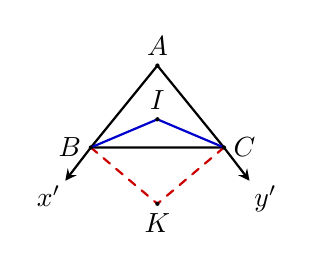
\begin{tikzpicture}[scale=0.65, >=stealth, line join=round, line cap=round]
  \coordinate (A) at (1.5, 2.3);
  \coordinate (B) at (0.2, 0.7);
  \coordinate (C) at (2.8, 0.7);
  \coordinate (I) at (1.5, 1.25);
  \coordinate (K) at (1.5, -0.4);
  
  \draw[thick] (A) -- (B) -- (C) -- cycle;
  \draw[thick, blue!80!black] (B) -- (I) -- (C);
  
  \draw[thick, ->] (B) -- (-0.3, 0.05) node[below left=-2pt] {$x'$};
  \draw[thick, ->] (C) -- (3.3, 0.05) node[below right=-2pt] {$y'$};
  
  \draw[thick, red!80!black, dashed] (B) -- (K) -- (C);
  
  \fill (A) circle (1.2pt) node[above] {$A$};
  \fill (B) circle (1.2pt) node[left] {$B$};
  \fill (C) circle (1.2pt) node[right] {$C$};
  \fill (I) circle (1.2pt) node[above] {$I$};
  \fill (K) circle (1.2pt) node[below] {$K$};
\end{tikzpicture}
\end{minipage}\par
\vspace{0.4mm}
\noindent\textit{Bài giải:}\dongkeHaiCot{9}
\\ \hline
\end{tabularx}

\vspace{1.5mm}

\noindent
\begin{tabularx}{\linewidth}{|X|}
\hline
\vspace{0.5mm}
\textbf{Câu 14 (0,5 điểm).} Tìm giá trị lớn nhất của biểu thức: $B = \dfrac{18}{|x - 2| + 6}$.\par
\vspace{0.4mm}
\noindent\textit{Bài giải:}\dongkeHaiCot{7}
\\ \hline
\end{tabularx}

\newpage
% =============================================================================
% ========================= TOAN 7 TUAN 09 BUOI 02 - MA DE 104 =================
% ========================= TRANG 1/2 ==========================================
% =============================================================================
\noindent
\begin{tabularx}{\linewidth}{|X|c|}
\hline
\textbf{PHIẾU KIỂM TRA ĐỊNH KỲ TOÁN 7 - TUẦN 09 - BUỔI 02} & \textbf{Mã đề: 104 - Trang 1/2} \\
\hline
\end{tabularx}

\vspace{1.2mm}

\noindent
\begin{tabularx}{\linewidth}{|p{3.2cm}|X|}
\hline
\centering\textbf{ĐIỂM SỐ} & \centering\textbf{LỜI NHẬN XÉT CỦA THẦY CÔ} \tabularnewline
\hline
\rule{0pt}{1.8cm} & \tabularnewline
\hline
\end{tabularx}

\vspace{1.5mm}
\noindent\textbf{Câu 1 (0,25 điểm).} Số đối của số hữu tỉ $\dfrac{2}{5}$ là: \shortans{-\dfrac{2}{5}}\par\vspace{2.7mm}
\noindent\textbf{Câu 2 (0,25 điểm).} Giá trị của căn bậc hai số học $\sqrt{225}$ bằng: \shortans{15}\par\vspace{2.7mm}
\noindent\textbf{Câu 3 (0,25 điểm).} Giá trị của biểu thức $|-8{,}6|$ bằng: \shortans{8{,}6}\par\vspace{2.7mm}
\noindent\textbf{Câu 4 (0,25 điểm).} Mỗi góc ngoài của một tam giác có số đo bằng: \shortans{\text{tổng 2 góc trong không kề}}\par\vspace{2.7mm}
\noindent\textbf{Câu 5 (0,25 điểm).} Cho $\Delta ABC$ có $\widehat{A} = 60^\circ, \widehat{B} = 45^\circ$. Số đo góc ngoài tại đỉnh $C$ là: \shortans{105^\circ}\par\vspace{2.7mm}
\noindent\textbf{Câu 6 (0,25 điểm).} Góc ngoài tại đỉnh $A$ của $\Delta ABC$ bằng $135^\circ$, biết $\widehat{B} = 70^\circ$. Số đo $\widehat{C}$ là: \shortans{65^\circ}\par\vspace{2.7mm}
\noindent\textbf{Câu 7 (0,25 điểm).} Tổng số đo ba góc ngoài tại ba đỉnh của tam giác bất kì là: \shortans{360^\circ}\par\vspace{2.7mm}
\noindent\textbf{Câu 8 (0,25 điểm).} Cho $\Delta MNP$ vuông tại $M$, góc ngoài tại đỉnh $N$ bằng $130^\circ$. Số đo góc $\widehat{P}$ là: \shortans{40^\circ}\par\vspace{2.7mm}
\noindent\textbf{Câu 9 (0,25 điểm).} Cho $\Delta ABC$ có $\widehat{A} = 50^\circ$, hai phân giác trong góc $B, C$ cắt nhau tại $I$. Số đo $\widehat{BIC}$ là: \shortans{115^\circ}\par\vspace{2.7mm}
\noindent\textbf{Câu 10 (0,25 điểm).} Mái nhà tam giác cân góc đỉnh $80^\circ$. Góc ngoài tại đỉnh ở chân mái bằng: \shortans{130^\circ}\par\vspace{2.7mm}
\vspace{0.2mm}
\noindent\textbf{Câu 11 (3,0 điểm). Thực hiện phép tính (hợp lý nếu có thể):}
\vspace{0.8mm}

\noindent
\begin{tabularx}{\linewidth}{|X|X|}
\hline
\oBaiTap[5]{a) (0,5 điểm)}{$\dfrac{5}{14} + \dfrac{4}{7} - \dfrac{1}{2}$} & 
\oBaiTap[5]{b) (0,5 điểm)}{$\dfrac{8}{13} \cdot \left(-\dfrac{3}{10}\right) + \dfrac{8}{13} \cdot \left(-\dfrac{7}{10}\right)$} \\
\hline
\oBaiTap[5]{c) (0,5 điểm)}{$\left(-\dfrac{3}{2}\right)^2 \cdot \dfrac{4}{9} - \sqrt{\dfrac{4}{25}}$} & 
\oBaiTap[5]{d) (0,5 điểm)}{$\left|-\dfrac{5}{9}\right| - \sqrt{\dfrac{16}{81}} + \dfrac{2}{9}$} \\
\hline
\oBaiTap[5]{e) (0,5 điểm)}{$\dfrac{10}{3} - \left[\dfrac{7}{6} - \left(\dfrac{2}{3} - \dfrac{1}{3}\right)\right]$} & 
\oBaiTap[5]{f) (0,5 điểm)}{$\dfrac{3^9 \cdot 2^6}{6^5 \cdot 9}$} \\
\hline
\end{tabularx}

\newpage
% =============================================================================
% ========================= TOAN 7 TUAN 09 BUOI 02 - MA DE 104 =================
% ========================= TRANG 2/2 ==========================================
% =============================================================================
\noindent
\begin{tabularx}{\linewidth}{|X|c|}
\hline
\textbf{TOÁN 7 - TUẦN 09 - BUỔI 02} & \textbf{Mã đề: 104 - Trang 2/2} \\
\hline
\end{tabularx}

\vspace{1.5mm}

\noindent\textbf{Câu 12 (2,0 điểm). Tìm số hữu tỉ $x$, biết:}
\vspace{0.8mm}

\noindent
\begin{tabularx}{\linewidth}{|X|X|}
\hline
\oBaiTap[5]{a) (0,5 điểm)}{$x + \dfrac{2}{9} = \dfrac{7}{18}$} & 
\oBaiTap[5]{b) (0,5 điểm)}{$\dfrac{5}{8}x - \dfrac{1}{3} = \dfrac{7}{24}$} \\
\hline
\oBaiTap[5]{c) (0,5 điểm)}{$\left(x + \dfrac{1}{5}\right)^2 = \dfrac{9}{25}$} & 
\oBaiTap[5]{d) (0,5 điểm)}{$\left|3x - \dfrac{1}{5}
ight| = \dfrac{7}{5}$} \\
\hline
\end{tabularx}

\vspace{1.5mm}

\noindent
\begin{tabularx}{\linewidth}{|X|}
\hline
\vspace{0.5mm}
\begin{minipage}[t]{0.67\linewidth}
\vspace{0pt}
\textbf{Câu 13 (2,0 điểm).} Cho tam giác $ABC$ có $\widehat{A} = 90^\circ$ (tam giác vuông tại $A$). Hai tia phân giác của hai góc trong $\widehat{B}$ và $\widehat{C}$ cắt nhau tại điểm $I$.\par\vspace{0.4mm}
\textbf{a)} (1,0 điểm) Tính số đo góc $\widehat{BIC}$.\par\vspace{0.4mm}
\textbf{b)} (1,0 điểm) Kéo dài cạnh $AB$ về phía $B$ được tia $Bx'$, kéo dài $AC$ về phía $C$ được tia $Cy'$. Hai tia phân giác của hai góc ngoài $\widehat{x'BC}$ và $\widehat{y'CB}$ cắt nhau tại điểm $K$. Tính số đo góc $\widehat{BKC}$.
\end{minipage}\hfill
\begin{minipage}[t]{0.31\linewidth}
\vspace{0pt}\centering
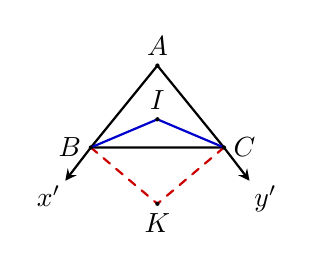
\begin{tikzpicture}[scale=0.65, >=stealth, line join=round, line cap=round]
  \coordinate (A) at (1.5, 2.3);
  \coordinate (B) at (0.2, 0.7);
  \coordinate (C) at (2.8, 0.7);
  \coordinate (I) at (1.5, 1.25);
  \coordinate (K) at (1.5, -0.4);
  
  \draw[thick] (A) -- (B) -- (C) -- cycle;
  \draw[thick, blue!80!black] (B) -- (I) -- (C);
  
  \draw[thick, ->] (B) -- (-0.3, 0.05) node[below left=-2pt] {$x'$};
  \draw[thick, ->] (C) -- (3.3, 0.05) node[below right=-2pt] {$y'$};
  
  \draw[thick, red!80!black, dashed] (B) -- (K) -- (C);
  
  \fill (A) circle (1.2pt) node[above] {$A$};
  \fill (B) circle (1.2pt) node[left] {$B$};
  \fill (C) circle (1.2pt) node[right] {$C$};
  \fill (I) circle (1.2pt) node[above] {$I$};
  \fill (K) circle (1.2pt) node[below] {$K$};
\end{tikzpicture}
\end{minipage}\par
\vspace{0.4mm}
\noindent\textit{Bài giải:}\dongkeHaiCot{9}
\\ \hline
\end{tabularx}

\vspace{1.5mm}

\noindent
\begin{tabularx}{\linewidth}{|X|}
\hline
\vspace{0.5mm}
\textbf{Câu 14 (0,5 điểm).} Tìm giá trị lớn nhất của biểu thức: $B = \dfrac{20}{|x - 4| + 5}$.\par
\vspace{0.4mm}
\noindent\textit{Bài giải:}\dongkeHaiCot{7}
\\ \hline
\end{tabularx}
\end{document}
